% Workflow diagram. Build: cd paper/figures && pdflatex diagram.tex  (done by paper/build.sh)
\documentclass[tikz,border=4pt]{standalone}
\usetikzlibrary{arrows.meta}
\begin{document}
\sffamily\small
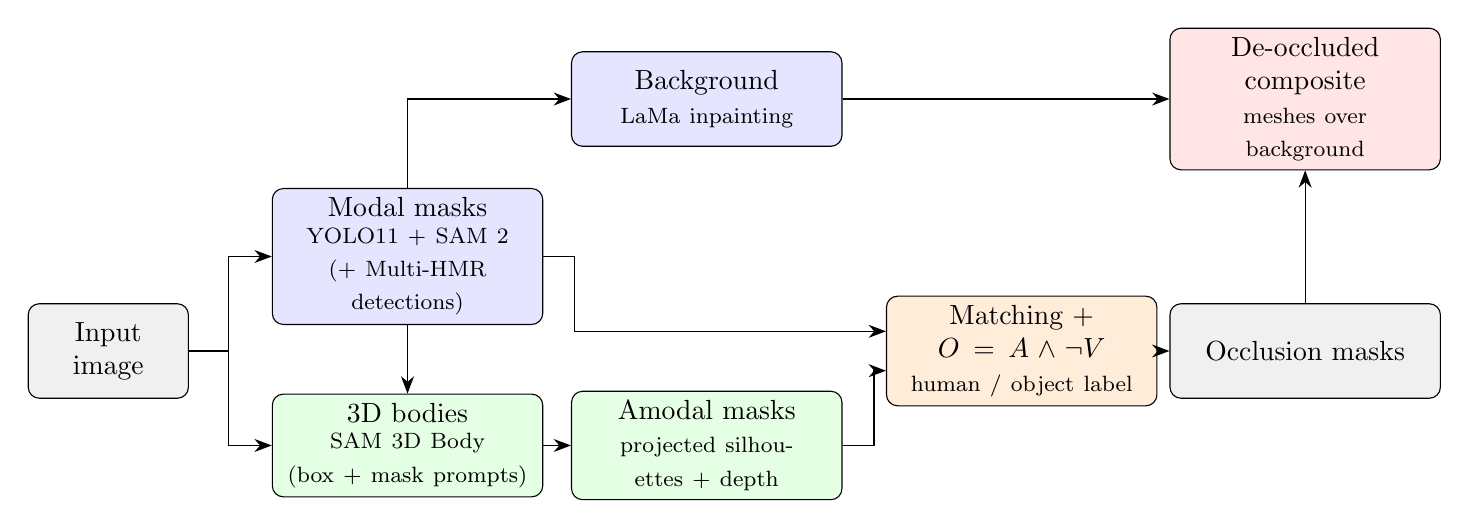
\begin{tikzpicture}[
  box/.style={draw, rounded corners, align=center, minimum height=12mm, text width=32mm, fill=#1},
  box/.default=white, >={Stealth[length=2.2mm]}]
  \node[box=gray!12, text width=18mm] (img) at (0,0) {Input image};
  \node[box=blue!10]   (modal) at (3.8,1.2) {Modal masks\\\footnotesize YOLO11 + SAM 2\\(+ Multi-HMR detections)};
  \node[box=green!10]  (hmr)  at (3.8,-1.2) {3D bodies\\\footnotesize SAM 3D Body\\(box + mask prompts)};
  \node[box=green!10]  (proj) at (7.6,-1.2) {Amodal masks\\\footnotesize projected silhouettes + depth};
  \node[box=orange!15] (occ)  at (11.6,0)   {Matching + $O = A \land \lnot V$\\\footnotesize human / object label};
  \node[box=gray!12]   (out)  at (15.2,0)   {Occlusion masks};
  \node[box=blue!10]   (bg)   at (7.6,3.2)  {Background\\\footnotesize LaMa inpainting};
  \node[box=red!10]    (comp) at (15.2,3.2) {De-occluded composite\\\footnotesize meshes over background};
  \draw[->] (img.east) -- ++(0.5,0) |- (modal.west);
  \draw[->] (img.east) -- ++(0.5,0) |- (hmr.west);
  \draw[->] (hmr) -- (proj);
  \draw[->] (modal) -- (hmr);
  \draw[->] (modal.east) -- ++(0.4,0) |- ([yshift=2.5mm]occ.west);
  \draw[->] (proj.east) -- ++(0.4,0) |- ([yshift=-2.5mm]occ.west);
  \draw[->] (occ) -- (out);
  \draw[->] (modal.north) |- (bg.west);
  \draw[->] (bg) -- (comp);
  \draw[->] (out) -- (comp);
\end{tikzpicture}
\end{document}
